\documentclass[aspectratio=169, ignorenonframetext]{beamer}
\usepackage{pgf}

\mode<article>{
  \usepackage{fullpage}

}

\mode<presentation>
{
%   \usetheme{Madrid}
%   \useinnertheme{circles}
  \setbeamertemplate{navigation symbols}{}
%   \usetheme[hideothersubsections, width=2.4cm]{Hannover}
%   \usetheme{Antibes}
%   \usetheme{Montpellier}
%   \usetheme{Singapore}
  \usetheme{Darmstadt}
%   \usecolortheme{seahorse}
%   \usecolortheme{orchid}
  \setbeamertemplate{footline}
  {%
%     \begin{beamercolorbox}{section in head/foot}
%       \usebeamercolor{bg}
       \hskip 1em \footnotesize \insertframenumber{} / \inserttotalframenumber%\hskip 41em \includegraphics[height = .5cm]{../../../../bilder/cc_by-nc_eu.png}
% % cc_by-nc_eu.png: 403x141 px, 72dpi, 14.22x4.97 cm, bb=0 0 403 141
%
% % bwslogo_3.png: 476x392 px, 300dpi, 4.03x3.32 cm, bb=0 0 114 94
%
%       %\hskip 5em
%       %       \input{../bilder/cc_by.png}
%       %\includegraphics[height=.5cm]{../../../../bilder/bwslogo_3.png}
%     \end{beamercolorbox}%
  }
  \usepackage{beamerfoils}
}
\usepackage[german]{babel}
\usepackage[utf8]{inputenc}
\usepackage{times}
\usepackage[T1]{fontenc}
\usepackage{pgf}
\usepackage{pgfpages}
\usepackage{eurosym}
\usepackage{graphicx}
\usepackage{amsmath}
\usepackage[siunitx,european]{circuitikz}
\usepackage{ulem}
\usepackage{listings}
\usepackage{svg}
%
\lstset{numbers=left, numberstyle=\tiny, stepnumber=2, numbersep=5pt, language = C++, alsolanguage=XML}
% \MyLogo{\includegraphics[height=1cm]{../../../../bilder/bwslogo_3.png}}
% % \includegraphics{../../bilder/bwslogo_3.png}
% % bwslogo_3.png: 476x392 px, 300dpi, 4.03x3.32 cm, bb=
%
\only<article>{
  \usepackage[colorlinks=true,linkcolor=blue,filecolor=magenta,urlcolor=cyan]{hyperref}
}

\only<presentation>{
  \usepackage{hyperref}
}


\title{Arbeitsunterlagen zu FOS Elektrotechnik, technische Informatik, Mechatronik Themenfeld 12.1}
\subtitle{Gleichstromnetzanalyse - Teil 1}
\date{V 0.5.1 \\ Stand: \today}%\\

\institute[BWS Hofheim]{Brühlwiesenschule, Hofheim}
\author{Thomas Maul}

\titlegraphic{Für eigene Teile gilt: 
\includegraphics[height=1cm]{cc_by-nc_eu.png}}

\begin{document}
  \only<article>{
    \maketitle
    \tableofcontents
    \clearpage
  }
  \begin{frame}<beamer>
    \titlepage
    % \hyperlink{Teil_2}{\beamerbutton{Go part 2}}
  \end{frame}
  % \AtBeginSection[] % Do nothing for \section*
  % {
  %   \begin{frame}<beamer>
  %     \frametitle{Inhalt}
  %     \tableofcontents[currentsection]
  %   \end{frame}
  % }
% \begin{frame}{Was bisher geschah}
%     \begin{itemize}
%         \item Atome und Elektronen
%         \item Ladungen im Sinne der Elektrotechnik
%         \item Gleichstrom und Wechselstrom
%         \item Widerstand, Strom, Spannung, Leistung
%     \end{itemize}
% \end{frame}


% \part{Themenfeld 12.1 - Gleichstromnetzanalyse}
\begin{frame}
  \partpage
  %   \tableofcontents[hidesubsections]
\end{frame}
\begin{frame}<beamer>
  \frametitle{Inhalt}
  \begin{columns}
    \column{.5\textwidth}
    \tableofcontents[sections={1-4},hidesubsections]%currentsection]
    ZAP = In der Themenliste der Abschlussprüfung genannt.
    \column{.5\textwidth}
    \tableofcontents[sections={5-},hidesubsections]%currentsection]
  \end{columns}
\end{frame}
\section[MaschenV]{Kreisstromverfahren (ZAP)}
Bei diesem Verfahren werden virtuelle Ströme berechnet. In Teilen der Schaltung, in denen nur ein Kreisstrom fließt, ist der Strom des Zweigs identisch zum Kreisstrom der Masche. Wenn mehrere virtuelle Kreisströme durch denselben Zweig fließen, müssen sie entsprechend der Zählrichtung addiert werden. Wenn die Zählrichtung beider Ströme identisch ist, werden sie addiert, sonst subtrahiert. Wenn ein Strom negativ ist, bedeutet dies, dass die Zählrichtung der Masche entgegen der tatsächlichen Stromrichtung ist.

\begin{frame}{Kreisstromverfahren - Baum I}
  \begin{columns}
    \begin{column}{.5\textwidth}\only<presentation>{
      \begin{figure}[htbp]
        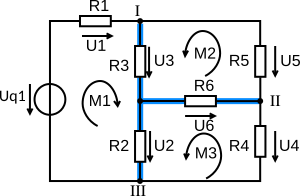
\includegraphics[scale=0.9,keepaspectratio=true]{messbruecke1_2}
        \caption{Messbrücke mit vollständigem Baum und Maschen}
      \end{figure}}
    \end{column}
    \begin{column}{.5\textwidth}
      \begin{enumerate}
        \item Baum festlegen (alle Knoten berühren, kein Umlauf).
        \item Maschen einzeichnen (Umlaufsinn ist willkürlich)
        \item Gleichungen aufstellen.
      \end{enumerate}
    \end{column}
  \end{columns}
\end{frame}

\begin{figure}[htbp]
  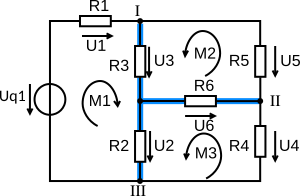
\includegraphics[scale=0.9,keepaspectratio=true]{messbruecke1_2}
  \caption{Messbrücke mit vollständigem Baum und Maschen}
  \label{KreisstromBaumMaschen-1}
\end{figure}

Im Bild \ref{KreisstromBaumMaschen-1} ist die Brückenschaltung gezeichnet. In Blau ist der sogenannte Baum eingezeichnet. Der Baum in der Schaltung ist eine Markierung, die alle Knoten berührt. Gleichzeitig darf sie keinen geschlossenen Umlauf bilden. Die Markierungen der Knoten (römische Zahlen) sind für die Maschenstrom- oder Kreisstromanalyse nicht relevant.

Bei der Festlegung des Baums sollte man berücksichtigen, dass Spannungsquellen immer außerhalb des Baums sein sollen. Es wäre hier auch möglich, statt des Ast mit R3 den Ast über R5 zu wählen. Ebenso wäre statt R2 ein Teil des Baums über R4 möglich. Im vorliegenden Baum wäre es auch möglich statt des Ast R6 entweder R5 oder R4 zu wählen.

Nach der Festlegung des Baums werden die Maschen festgelegt. Eine Masche besteht immer aus einer Sehne, einem Teil der Schaltung, der nicht zum Baum gehört und den Ästen des Baums um den Umlauf zu schließen. Masche M1 besteht aus der Sehne mit der Quelle Uq1 und R1. Zusätzlich sind die Äste mit R3 und R2 Teil der Masche.

Der Umlaufsinn der Masche ist frei wählbar. Bei Maschen, die eine Quelle beinhalten sollte man den Umlaufsinn entgegen dem Zählpfeil der Quelle (Zählpfeil hier nach unten, daher sollte der Umlauf an der Stelle nach oben verlaufen). Bei den Maschen 2 und 3 ist der Umlaufsinn frei wählbar.

\begin{frame}{Kreisstromverfahren - Baum II}
  \begin{columns}
    \begin{column}{.5\textwidth}\only<presentation>{
      \begin{figure}[htbp]
        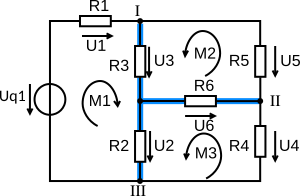
\includegraphics[scale=0.9,keepaspectratio=true]{messbruecke1_2}
        \caption{Messbrücke mit vollständigem Baum und Maschen}
      \end{figure}}
    \end{column}
    \begin{column}{.5\textwidth}
      Gleichungssystem
      \begin{enumerate}
        \item Hauptdiagonale: Rs in der Masche
        \item Nebendiagonalen: Verbindungs-Rs
        \item Quelle in Quellen-Vektor
      \end{enumerate}
    \end{column}
  \end{columns}
\end{frame}

Nach der Festlegung der Maschen werden die Widerstände in einer Matrix notiert. Auf der Hauptdiagonalen (von links oben nach rechts unten) werden die Widerstände der Maschen eingetragen. An Position 1-1 (links oben stehen die Widerstände der Masche 1, in der Mitte (Position 2-2) die Widerstände der Masche 2 und in der Position 3-3 die Widerstände der Masche 3.

An den anderen Positionen werden die Koppelwiderstände notiert. Masche 1 und Masche 2 haben den Koppelwiderstand R3, da in beiden Maschen nur R3 gemeinsam ist. Das Vorzeichen für R3 ist von den Umlaufrichtungen der beteiligten Maschen abhängig. Wenn die Umlaufrichtung (am betreffenden Widerstand / Ast) gleich ist, wird der Widerstand mit positiven Vorzeichen eingetragen. Wenn die Umlaufrichtungen gegenläufig sind, wird der Widerstand mit negativem Vorzeichen eingetragen. In Zeile 1, Spalte 2 wird der Widerstand (oder die Widerstände) eingetragen, mit denen die Maschen 1 und 2 verbunden sind\footnote{Die Widerstände im Baum-Zweig / den Baum-Zweigen, die die beiden Maschen gemeinsam haben.} Zeile 1, Spalte 3 ist die Kopplung von Masche 1 und Masche 3. Allgemein kann man sagen die Zeile bestimmt die eine Masche, die einen gemeinsamen Baum-Zweig haben\footnote{es können auch mehrere Zweige im Baum sein.}. Die Spalte bestimmt die zweite Masche der Kopplung.

Die "`untere Hälfte"' der Matrix (unten links von der Hauptdiagonalen) wird über die Hauptdiagonale gespiegelt. (Spalte 1, Zeile 3 wird von Zeile 1, Spalte 3 kopiert, etc.)

Anschließend werden der Vektor für die Maschenströme (hier $\text{I}_{M1}$ bis $\text{I}_{M3}$) erstellt und - rechts vom Gleichheitszeichen - der Vektor mit den Spannungsquellen. Wenn in einer Masche keine Quelle vorhanden ist, wird dort 0 eingetragen. (siehe Gleichungssystem, unten)

\begin{frame}{Kreisstromverfahren - Gleichungssystem}
  \begin{columns}
    \begin{column}{.5\textwidth}
      \begin{figure}[htbp]
        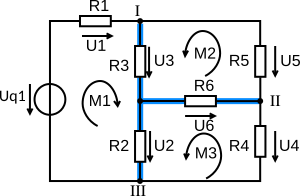
\includegraphics[scale=0.9,keepaspectratio=true]{messbruecke1_2}
        \caption{Messbrücke mit vollständigem Baum und Maschen}
      \end{figure}
    \end{column}
    \begin{column}{.5\textwidth}
      Gleichungssystem

        $\left( \begin{array}{rrrrrr}
          \text{R}1+\text{R}2+\text{R}3 &     \text{R}3  & \text{R}2  \\
          \text{R}3 & \text{R}3+\text{R}5+\text{R}6     & -\text{R}6   \\
          \text{R}2  & -\text{R}6      &   \text{R}2+\text{R}4+\text{R}6
\end{array}\right) *
\left(\begin{array}{c}
  \text{I}_{M1}\\
  \text{I}_{M2}\\
  \text{I}_{M3}
      \end{array} \right)
= \left( \begin{array}{c}
  \text{U}_{q1}\\
 0\\
 0\\
\end{array}\right)
$\label{LGSBrueckenschaltung1}
    \end{column}
  \end{columns}
\end{frame}

Das Gleichungssystem kann per Hand gelöst werden. Alternativ ist eine Lösung mit einem geeigneten Taschenrechner oder z.B. octave auf dem Computer möglich. Octave ist open source.

% \only<presentation>{
\begin{frame}{Kreisstromverfahren - Gleichungssystem}
       % $\left(
       $\begin{array}{crrrrrr}
        & \text{M1}& \text{M2}& \text{M3}\\
        \text{M1}\  \vline & \text{R}1+\text{R}2+\text{R}3 &     \text{R}3  & \text{R}2 \vline \\
        \text{M2} \ \vline & \text{R}3 & \text{R}3+\text{R}5+\text{R}6     & -\text{R}6 \vline \\
        \text{M3} \ \vline & \text{R}2  & -\text{R}6      &   \text{R}2+\text{R}4+\text{R}6 \vline
\end{array}%\right)
*
\left(\begin{array}{c}
  \text{I}_{M1}\\
  \text{I}_{M2}\\
  \text{I}_{M3}
      \end{array} \right)
= \left( \begin{array}{c}
  \text{U}_{q1}\\
 0\\
 0\\
\end{array}\right)
$

LGS lösen:

\begin{itemize}
 \item per Hand - z.B. gaußsches Eliminationsverfahren\\ Matrix und Spannungs-Vektor in Dreiecksform bringen.
 \item im Taschenrechner - LGS Solver\\
 Matrix und Spannungsvektor eintippen.\\ Ergebnis ist Strom Vektor (von oben nach unten).
 \item mit dem PC z.B. octave (open source) - Eingabe vergleichbar mit Taschenrechner
\end{itemize}
\end{frame}%}

Die Eintragungen M1, M2 und M3 sind zusätzlich, als Hinweis eingetragen. Sie gehören nicht zum Gleichungssystem / der Matrix.
An den Kreuzungen stehen zwei unterschiedliche Informationen:

\begin{itemize}
 \item Hauptdiagonale (M1/M1, M2/M2, M3/M3): hier sind die Widerstände der jeweiligen Masche eingetragen.
 \item Nebendiagonalen (z. B. M1/M2) hier sind die Widerstände eingetragen, die sich zwei Maschen teilen. Bei gleicher Stromrichtung an dem Widerstand wird der Widerstand mit positivem Vorzeichen eingetragen (z. B. M1/M2: R3), bei unterschiedlichen Stromrichtungen wird der Widerstand mit negativen Vorzeichen eingetragen (z. B. M2/M3: -R6).
\end{itemize}

Die Eintragungen der Nebendiagonalen sind an der Hauptdiagonalen gespiegelt. (M1/M2 ist identisch zu M2/M1).
\end{document}

